\documentclass[12pt, letterpaper]{article}
\usepackage[utf8]{inputenc}
\usepackage{graphicx}
\usepackage{floatrow}

\usepackage[margin=2cm]{geometry} 



\renewcommand*\contentsname{Indholdsfortegnelse}


\begin{document}

\begin{titlepage}

\newcommand{\HRule}{\rule{\linewidth}{0.5mm}} % Defines a new command for the horizontal lines, change thickness here

\center % Center everything on the page
 
%----------------------------------------------------------------------------------------
%	HEADING SECTIONS
%----------------------------------------------------------------------------------------

\textsc{\LARGE Aarhus universitet}\\[1.5cm] % Name of your university/college
\textsc{\Large DSB}\\[0.5cm] % Major heading such as course name
\textsc{\large Semester 3}\\[0.5cm] % Minor heading such as course title

%----------------------------------------------------------------------------------------
%	TITLE SECTION
%----------------------------------------------------------------------------------------

\HRule \\[0.4cm]
{ \huge \bfseries Mini-projekt - Del 4}\\[0.4cm] % Title of your document
\HRule \\[1.5cm]
 
%----------------------------------------------------------------------------------------
%	AUTHOR SECTION
%----------------------------------------------------------------------------------------

% If you don't want a supervisor, uncomment the two lines below and remove the section above
\Large \emph{Studerende:}\\[1cm]
Mette \textsc{Hammer Nielsen-Kudsk - Studienr: 201408391}\\[0,5cm] % Your name
Martin \textsc{Banasik - Studienr: 201408398}\\[0,5cm] % Your name
Finja \textsc{Jette Ralfs - Studienr: 201303659}\\[0,5cm] % Your name
%----------------------------------------------------------------------------------------
%	DATE SECTION
%----------------------------------------------------------------------------------------

{\large December 3, 2015}\\[1,2cm] % Date, change the \today to a set date if you want to be precise

%----------------------------------------------------------------------------------------
%	LOGO SECTION
%----------------------------------------------------------------------------------------


\includegraphics[scale=0.5]{billeder/au}\\ % Include a department/university logo - this will require the graphicx package
 
 %\includegraphics[width=0.6\textwidth]{figurer/ASE}~\\[1cm]
%----------------------------------------------------------------------------------------

\vfill % Fill the rest of the page with whitespace


\end{titlepage}

\tableofcontents
\newpage


\section{Teori}
Dette miniprojekt er lavet med teori og viden fra hele dette semester. Derfor gentager vi ikke teoriafsnittet, men referer til vores tidligere miniprojekter.

\section{Valg af signal}
Miniprojektet går ud på at hive alle dele fra hele semesteret ind i opgaven. Derfor er det vigtigt at vælge et signal, som passer til de forskellige ting. Vi har haft mange forskellige overvejelser om hvorvidt vi skulle vælge et EEG-signal, et signal med støj fra en støvsuger eller et støjfyldt musiksignal. \\
Vi har valgt at arbejde med et støjfyldt musiknummer, da vi menter at vi kan hive rigtig mange forskellige ting, fra DSB undervisningen, ind. 
Vi har valgt et musiknummer fra Henry Mancini, der er vinyl. Derfor er der en masse vinyl skratten, så vi kan filtrere alle flimre og skrat fra.   

\section{Analyse af Henry Mancini}
Tidsdomæne ufiltreret. Her ser vi signalet i tidsdomænet. 
\begin{figure}[H]
           \includegraphics[width=\linewidth]{billeder/VinylUfiltreret}	   							\caption{Tidsdomæne ufiltreret}
\end{figure}

Her ser vi vores signal i frekvens domænet. Her kan vi se hvilket støj vi skal have fjernet fra vores signal. Vi kan se en høj søjle ved 2000 Hz. Det forsøger vi at fjerne. 
\begin{figure}[H]
           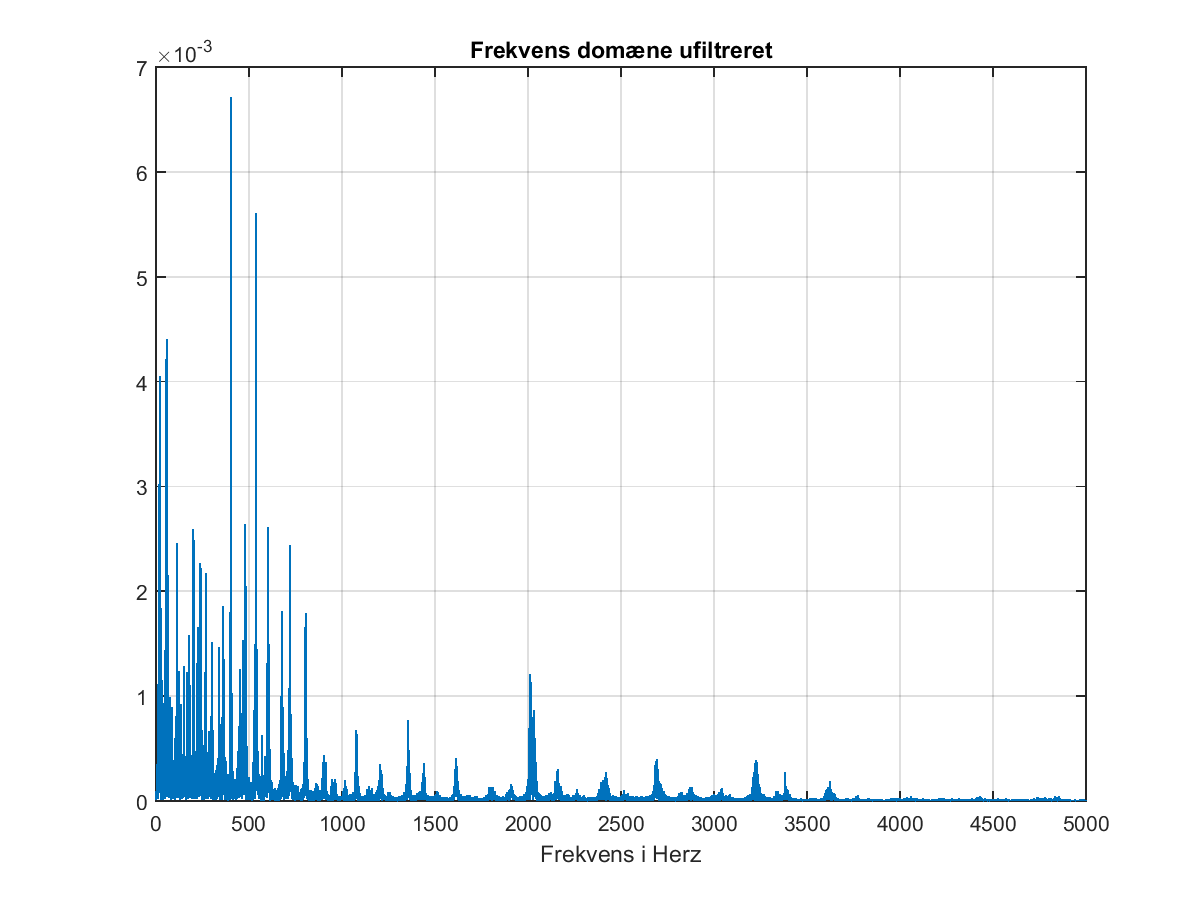
\includegraphics[width=\linewidth]{billeder/Vinylfrekvensd}	   							\caption{Frekvensdomæne ufiltreret}
\end{figure}

\newpage
Det gør vi ved hjælp af et FIR Båndstop filter med en knækfrekvens på 1990 Hz til 2070 Hz. Vi kan se herunder i frekvensdomænet, at vi vha. båndstop filteret har fået fjernet støjen: 
\begin{figure}[H]
           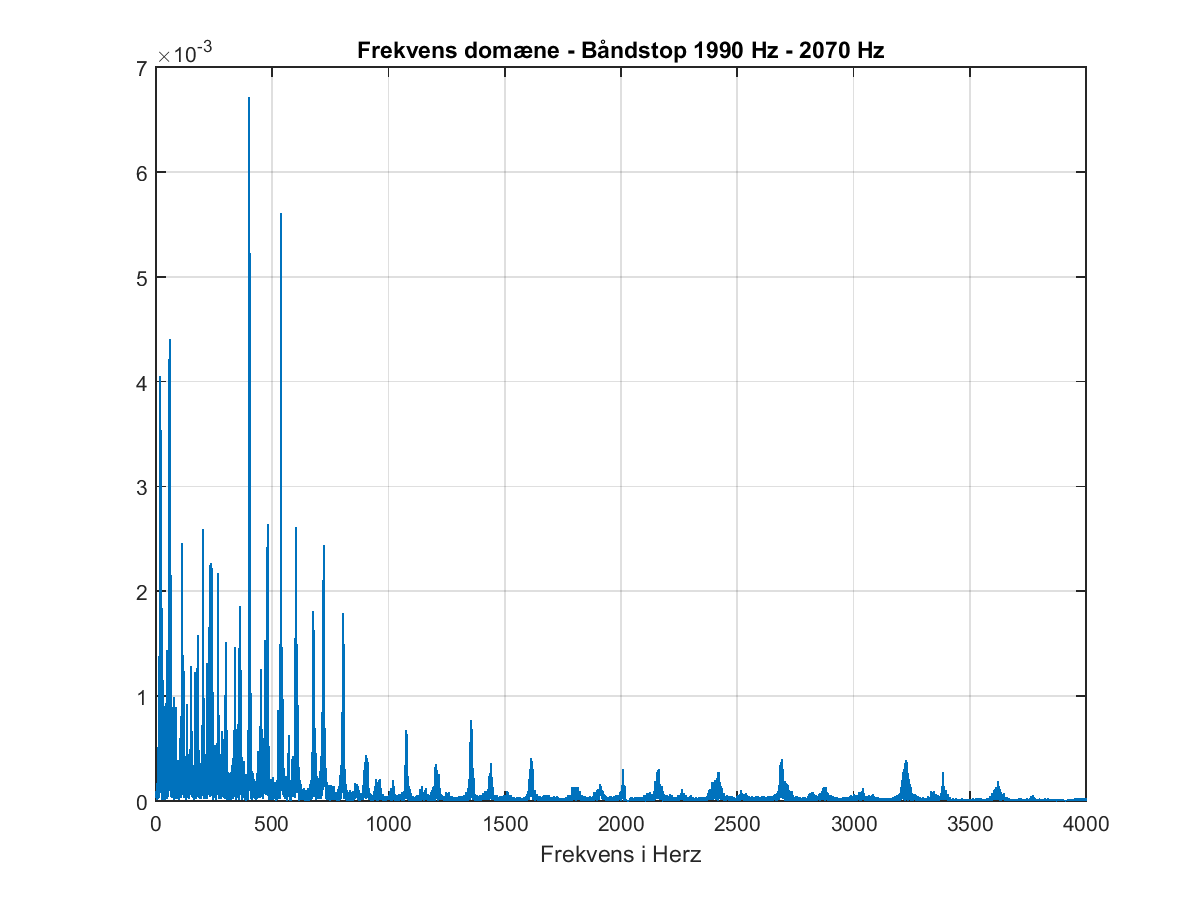
\includegraphics[width=\linewidth]{billeder/VinylBS1990}	   							\caption{Frekvensdomæne - Båndstop filter med knækfrekvens på 1990 Hz til 2070 Hz. }
\end{figure}

\newpage
Nu retter vi blikket mod starten af signalet, hvor vi kan se der er høje støjsøjler. Vi vil derfor igen benytte os af et båndstop filter på en knækfrekvens 390 Hz til 420 Hz. Herunder kan det ses at vi har fået fjernet støjen: 
\begin{figure}[H]
           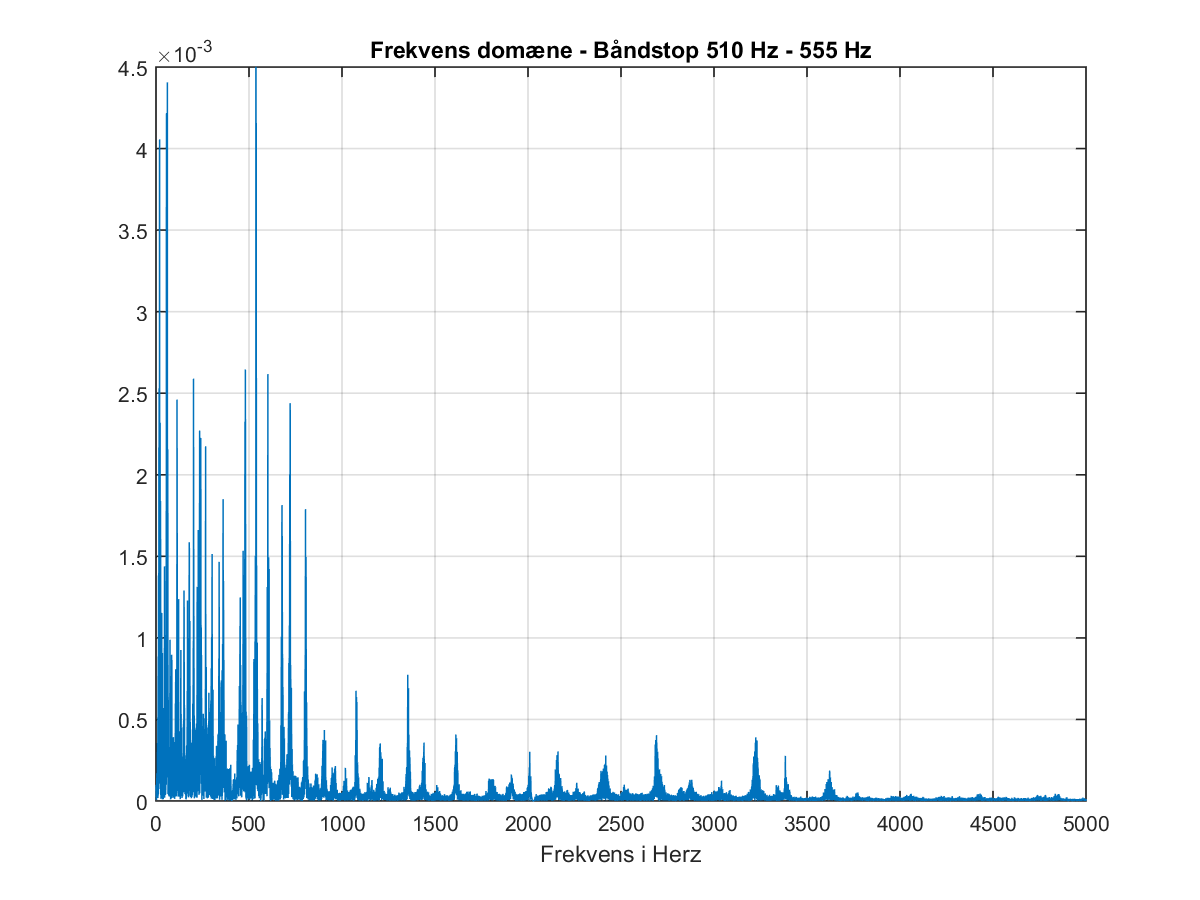
\includegraphics[width=\linewidth]{billeder/VinylBS390}	   							\caption{Frekvensdomæne - Båndstop filter med knækfrekvens på 390 Hz til 420 Hz.}
\end{figure}

\newpage
Det vi lægger mærke til nu er den højeste søjle af dem alle, der ligger ved en frekvens på 500 Hz. Derfor laver vi et båndstop filter med en frekvens på 510 Hz til 555 Hz. Vi kan igen se på billedet herunder at vi får fjernet støjen: 
\begin{figure}[H]
           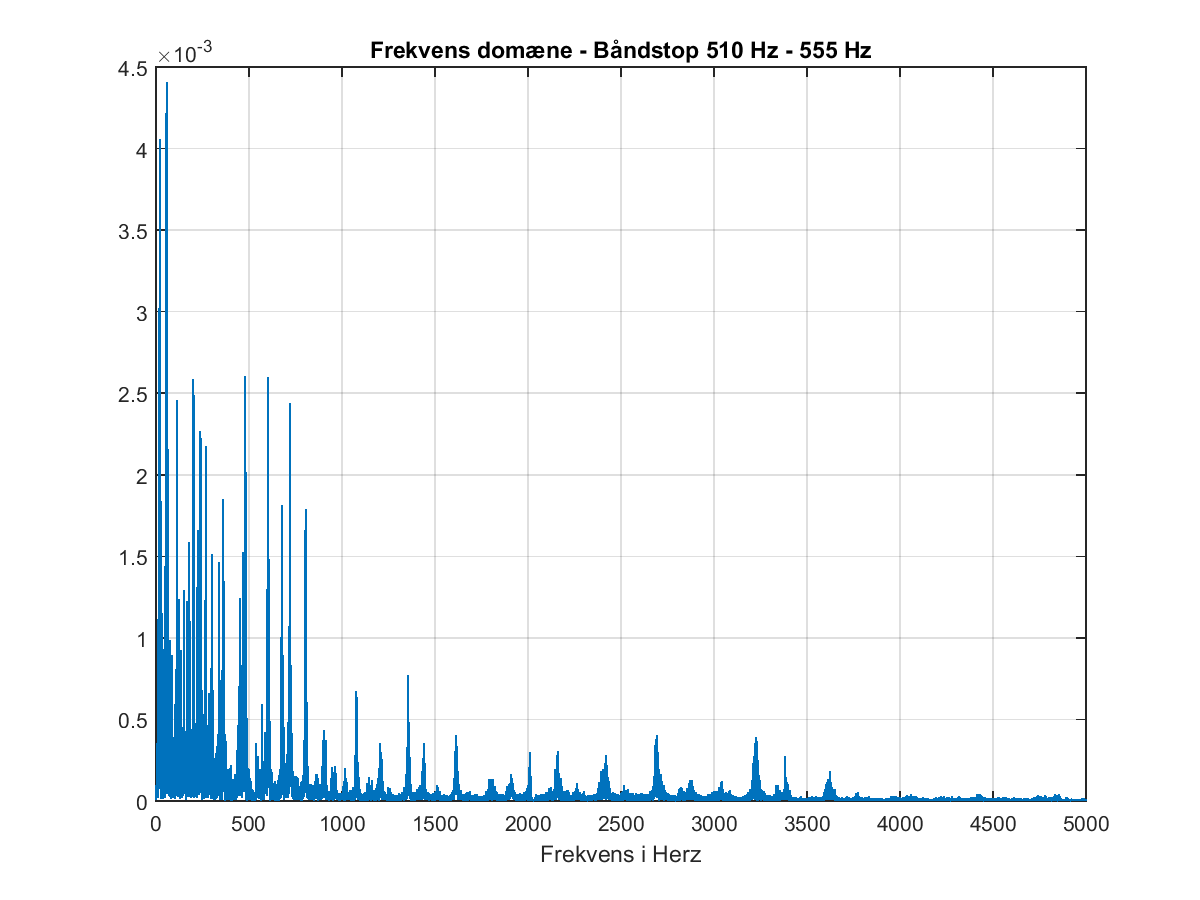
\includegraphics[width=\linewidth]{billeder/VinylBS510}	   							\caption{Frekvensdomæne - Båndstop filter med knækfrekvens på 510 Hz til 555 Hz.}
\end{figure}

\newpage
Vi ser nu endnu en høj støjsøjle ved ca. 50 Hz. Dette fjernes på samme måde med et Båndstop filter med en knækfrekvens på 50 Hz til 70 Hz. Støjen ses fjernet herunder: 
\begin{figure}[H]
           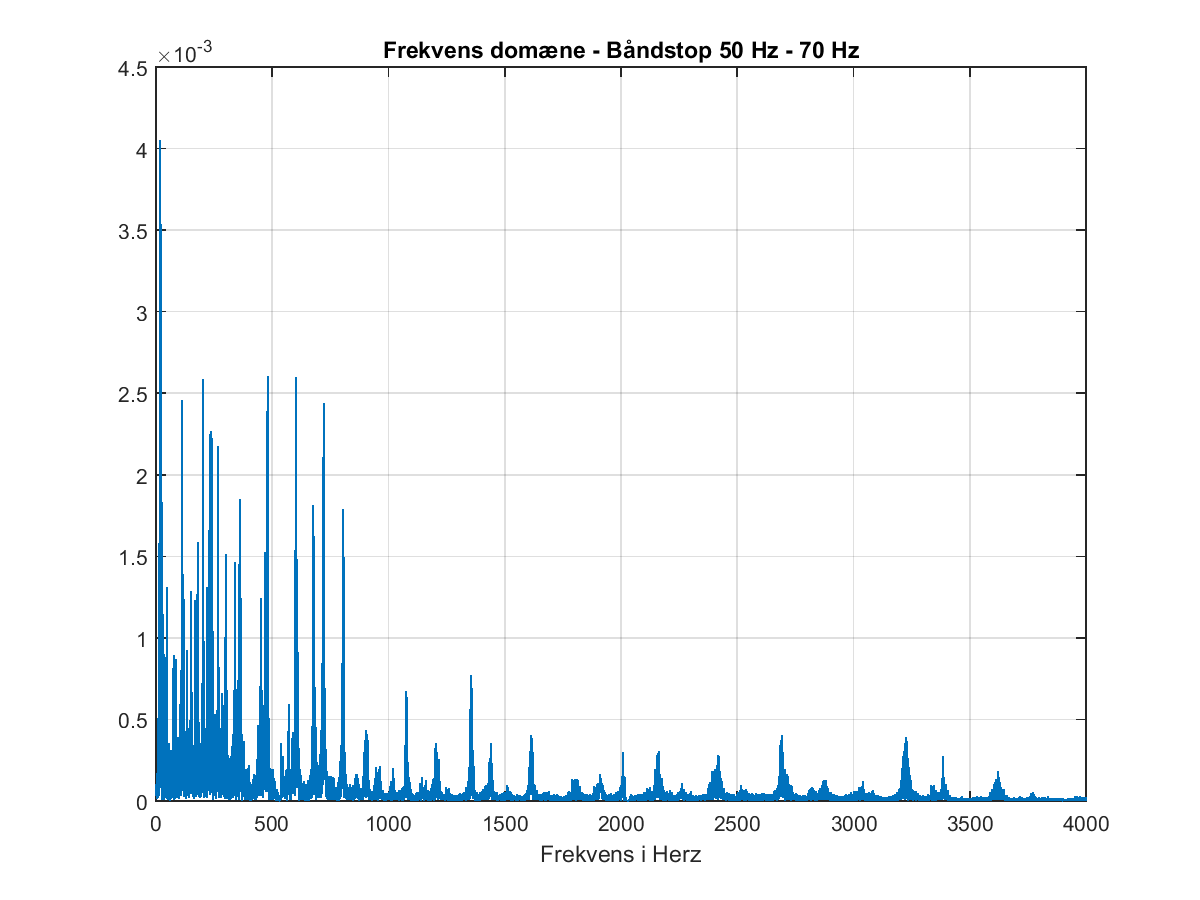
\includegraphics[width=\linewidth]{billeder/VinylBS50}	   							\caption{Frekvensdomæne - Båndstop filter med knækfrekvens på 50 Hz til 70 Hz.}
\end{figure}

\newpage
Hvis man kigger godt efter kan man nu helt i startet se endnu en søjle. 
Denne gang bliver båndpas filterets knækfrekvens på 1 Hz til 50 Hz. 
\begin{figure}[H]
           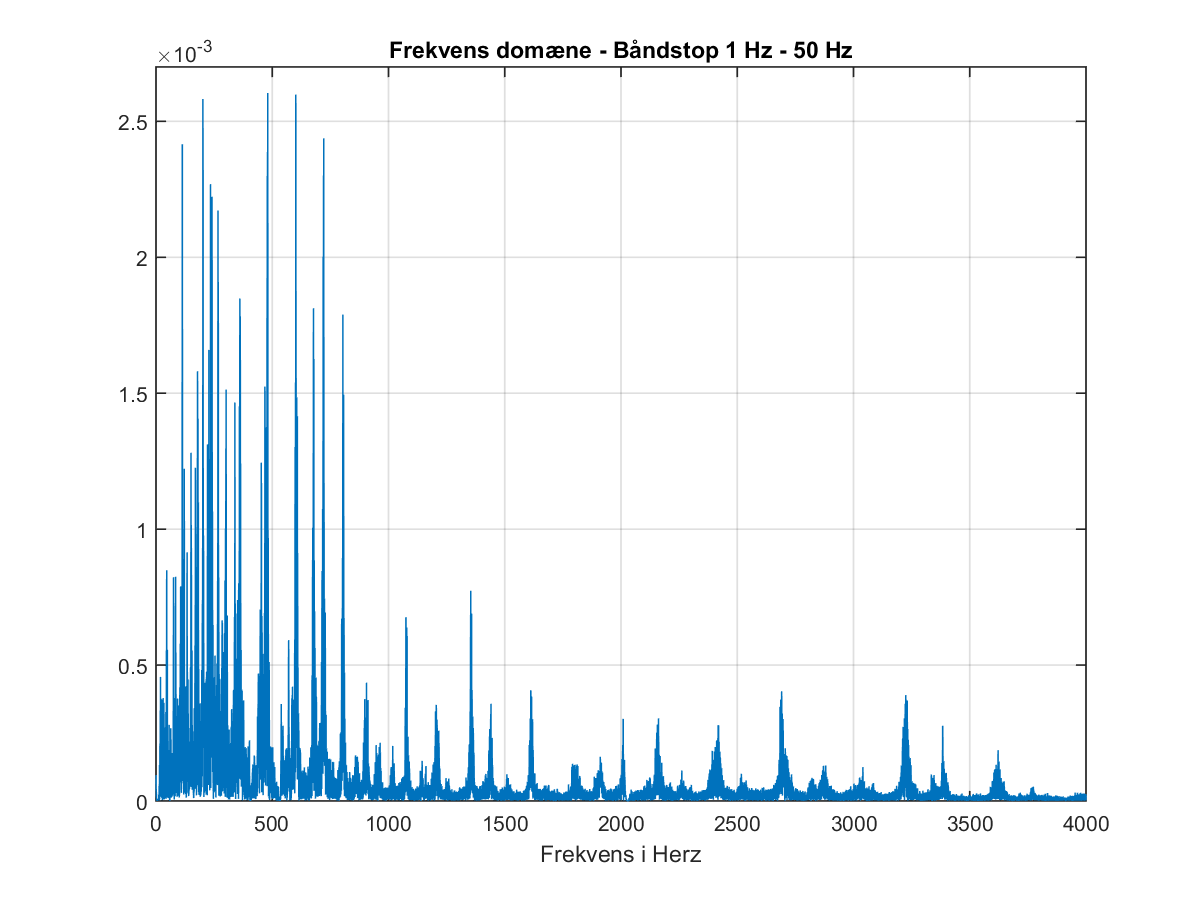
\includegraphics[width=\linewidth]{billeder/VinylBS1}	   							\caption{Frekvensdomæne - Båndstop filter med knækfrekvens på 1 Hz til 50 Hz. }
\end{figure} 

\newpage
Vi ser rigtig meget støj på alle frekvenser efter 3500 Hz. Dette fjerne vi med et IIR lavpas filter med en knækfrekvens på 3500 Hz. Her under kan vi se signalet med alle filtrene. 
\begin{figure}[H]
           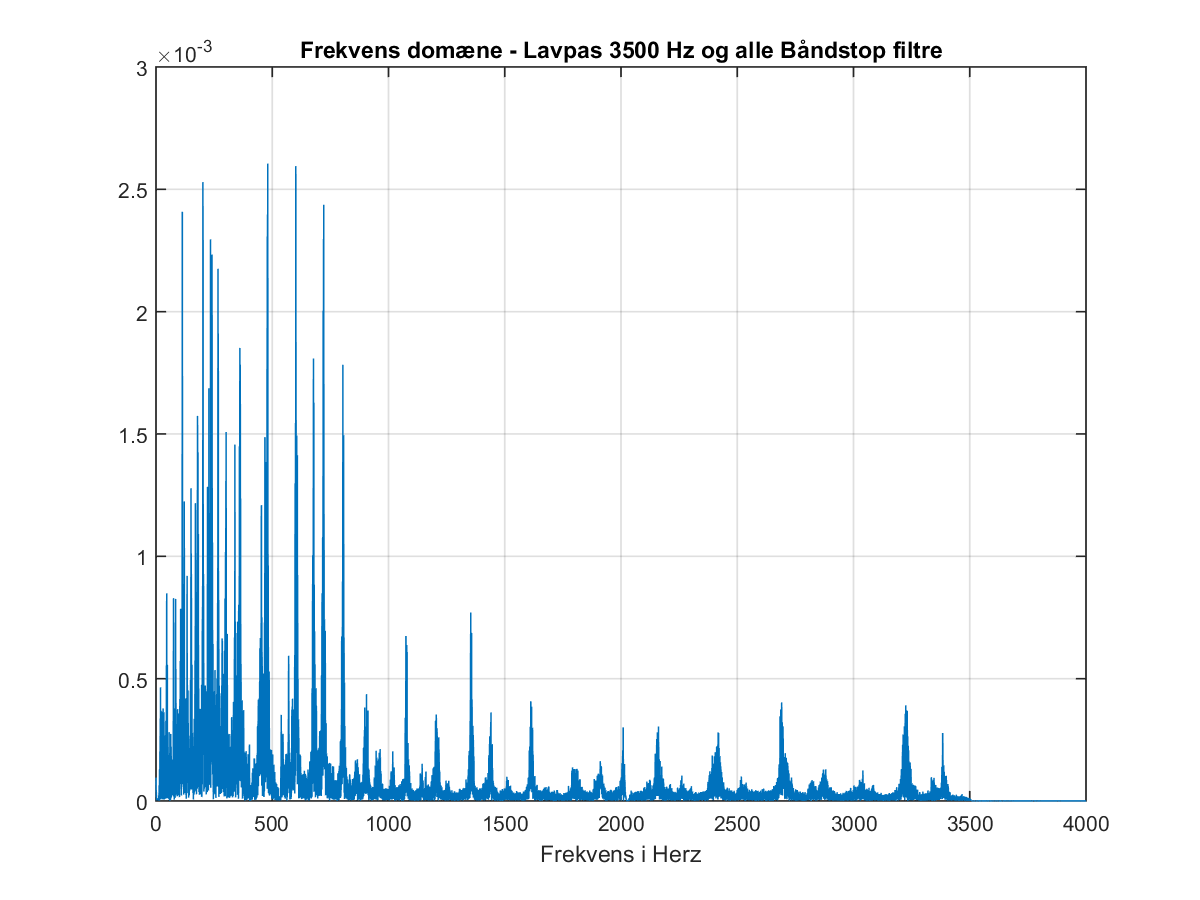
\includegraphics[width=\linewidth]{billeder/VinylLP3500}	   							\caption{Frekvensdomæne - Lavpas filter med knækfrekvens på 3500 Hz}
\end{figure} 

\newpage
Til sidst vil vi gerne se tidsdomænet igen, men denne gang med alle vores filtre lagt ovenpå. Vi kan se at utrolig meget af støjen er blevet fjernet og når vi selv lytter til signalet før filtreringen og efter filtreringen, så kan vi tydeligt høre at den vinyl skratrende lyd er blevet fjernet. Dejligt at høre!!!  
\begin{figure}[H]
           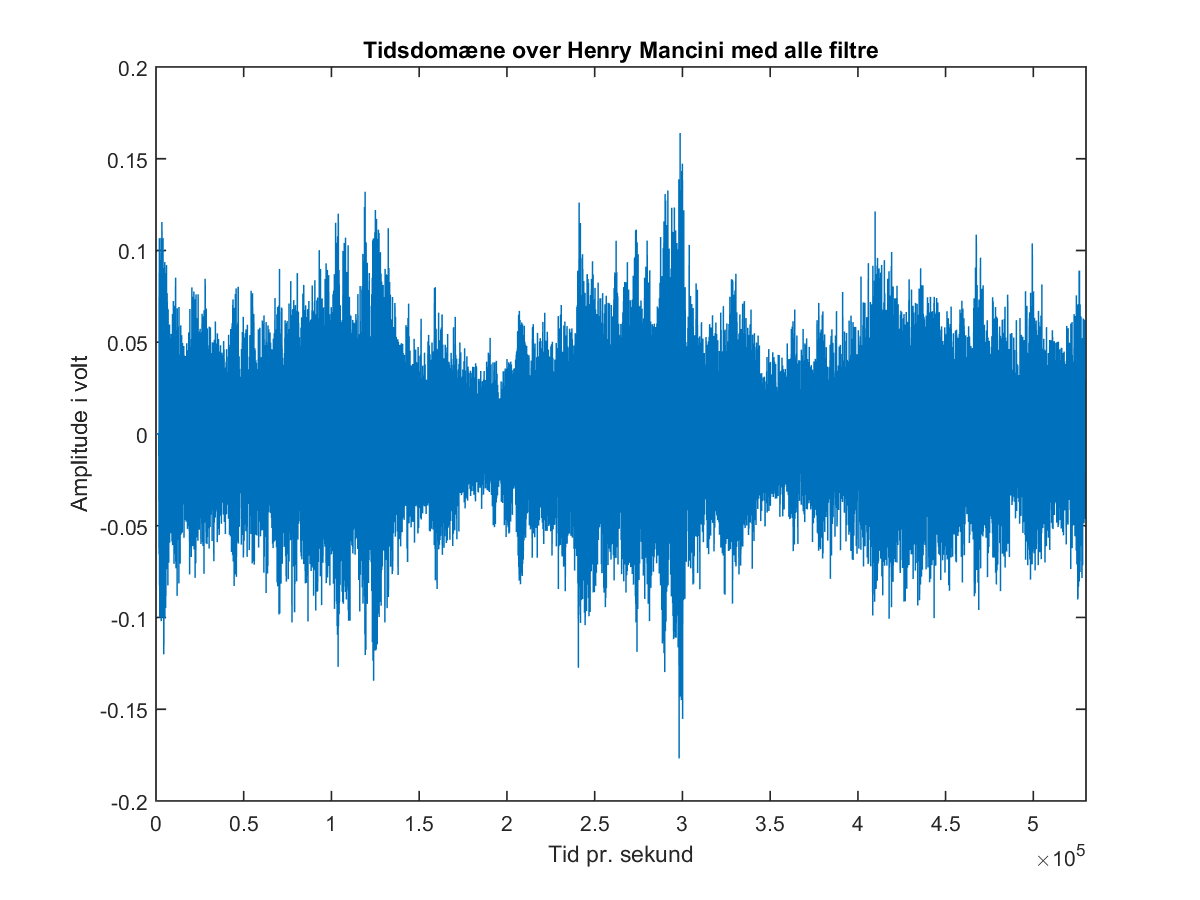
\includegraphics[width=\linewidth]{billeder/Vinyltidfiltreret}	   							\caption{Tidsdomæne filtreret}
\end{figure} 

\newpage
Hvis vi lige skal sammenligne i tidsdomænet, så kan man her virkelig se alt vi har fået dæmpet. 
\begin{figure}[H]
           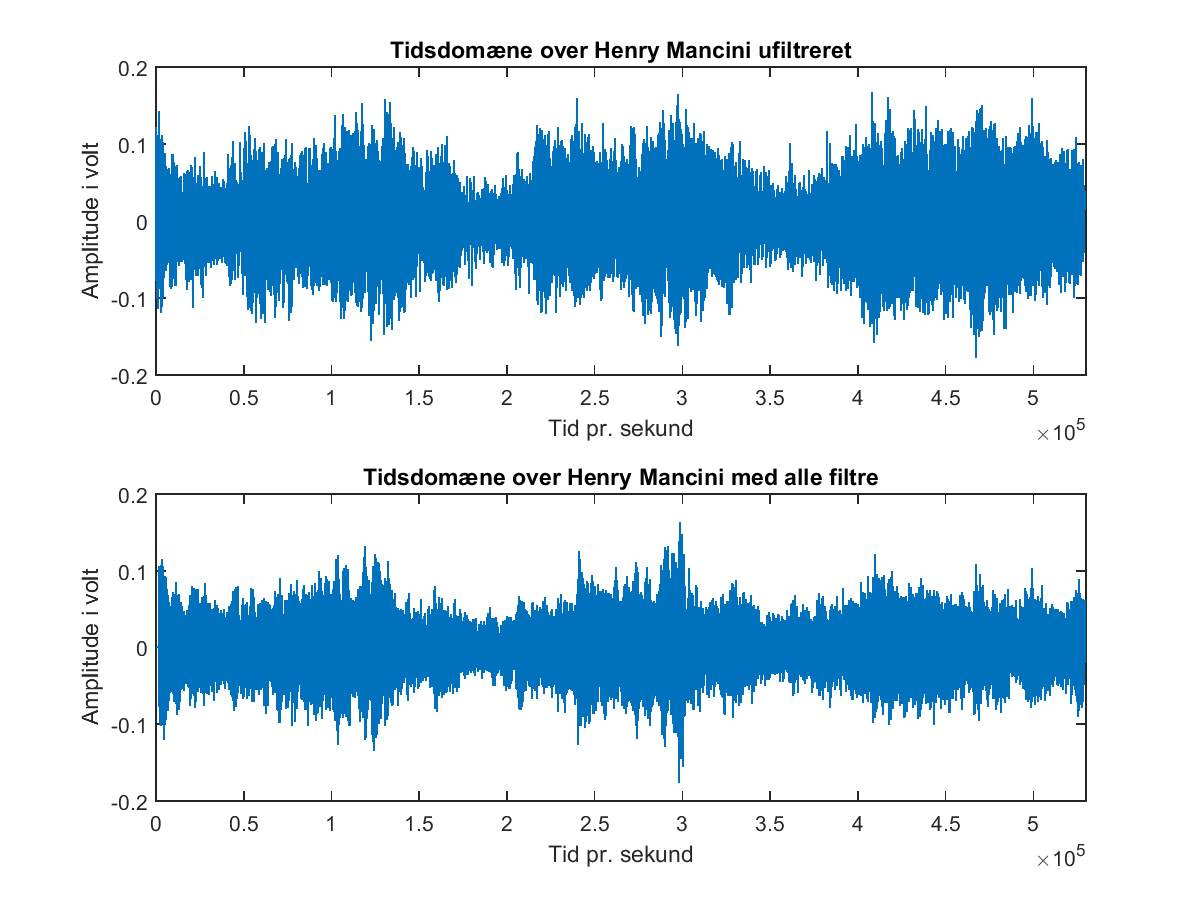
\includegraphics[width=\linewidth]{billeder/Vinylsamtid}	   							\caption{Sammenligning af tidsdomænet}
\end{figure} 

\newpage
Hvis vi ønsker at se sammenligningen i frekvensdomænet, kan vi også her se alt vi har fået fjernet. 
\begin{figure}[H]
           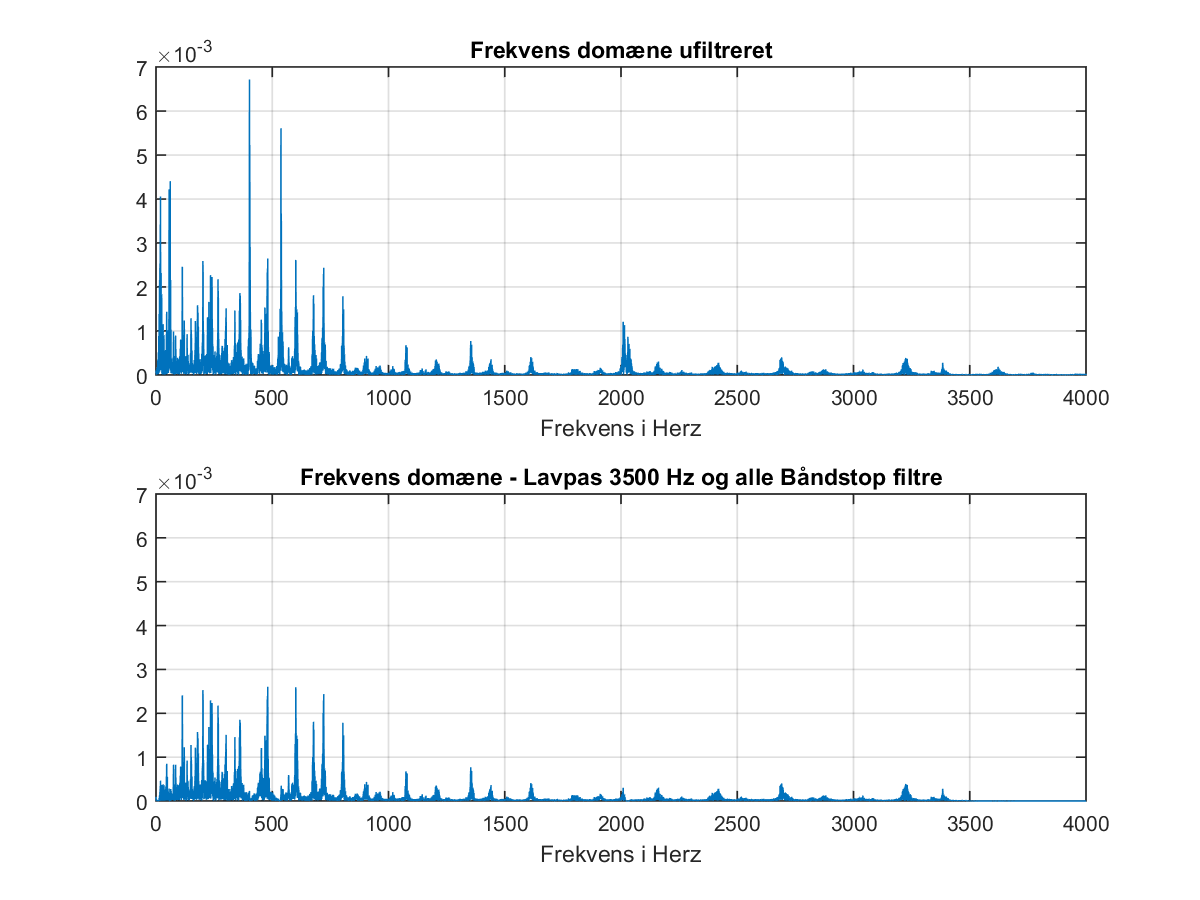
\includegraphics[width=\linewidth]{billeder/Vinylsamdom}	   							\caption{Sammenligning af frekvensdomænet}
\end{figure}

\newpage
Vi vil nu gerne se ændringen i tidsdomænet ordenligt. Det sorte signal er det ufiltrerede og det røde er det filtrerede. Vi kan se alt der vi har fået fjernet her: 
\begin{figure}[H]
           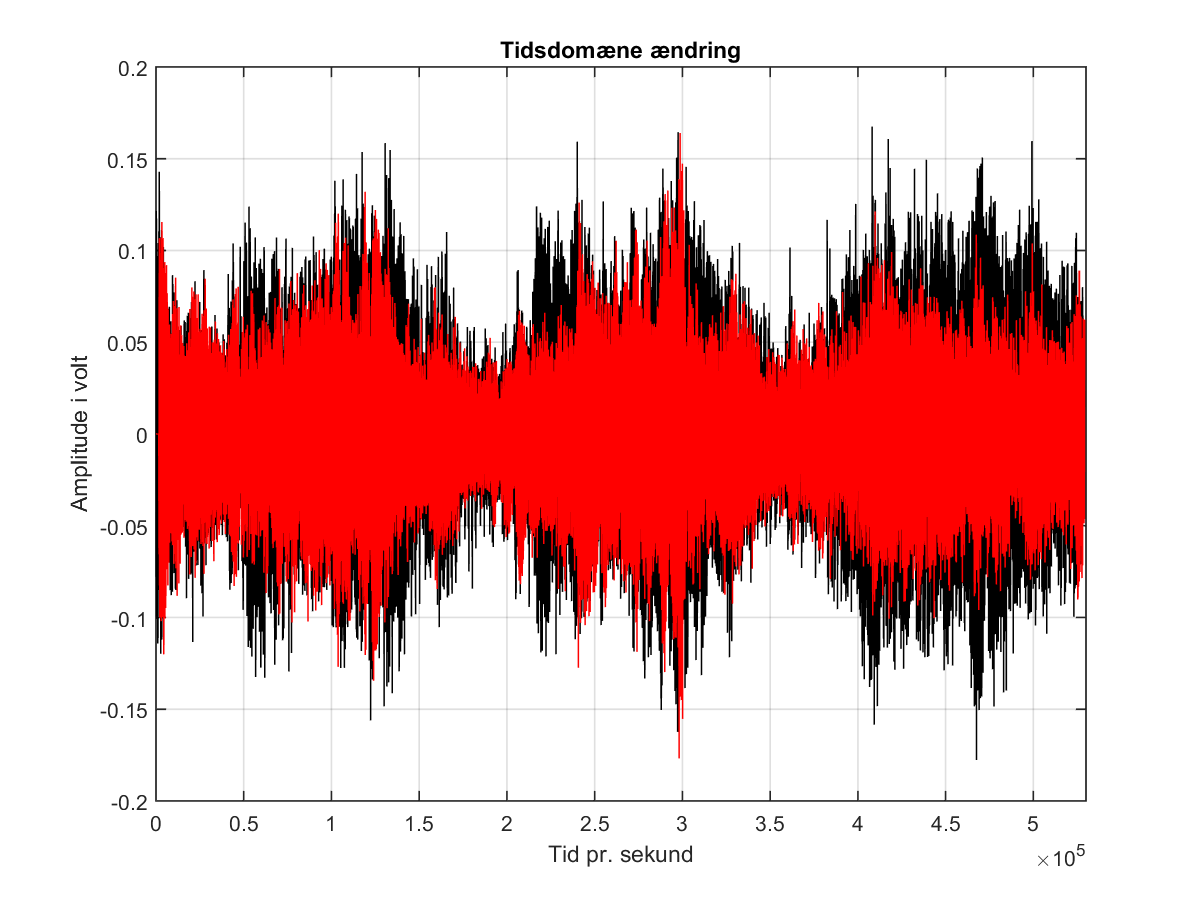
\includegraphics[width=\linewidth]{billeder/Vinyltidsdo}	   							\caption{Tidsdomæne ændringen efter alle filtre}
\end{figure}

\newpage
For bedre at se hvad vi præcis har fået fjernet, så ligger vi alle signalerne i frekvensdomænet oveni hinanden med forskellige farver. Så kan vi tydeligt se præcis hvilke spikes vi har fået fjernet. Det endelige signal er det sorte. Så alle de farvede spikes er det vi har fået fjernet. 
\begin{figure}[H]
           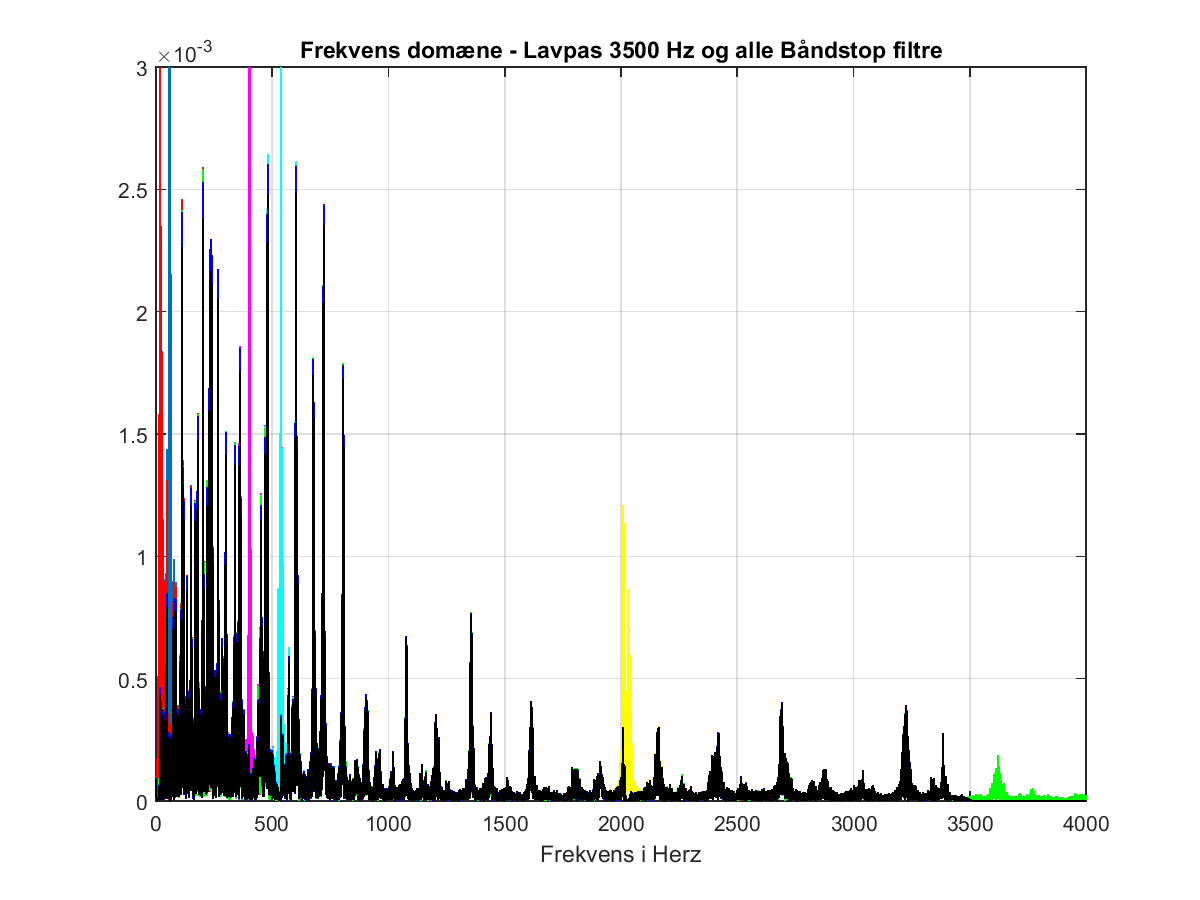
\includegraphics[width=\linewidth]{billeder/Vinyldom}	   							\caption{Alle filtre i frekvensdomænet.}
\end{figure}


\section{Fremtidigt arbejde}
Vi har lært at lave og forstå FIR og IIR filtre. Vi forstår foldning af filtre. Vi forstår og kan lave DFT på et signal og henholdsvis IDFT. 
Vi kan analysere, vurderer og forstå hvad, der sker med signaler når vi har benyttet filtre, DFT osv. Vi kan aflæse på frekvensdomæner hvad, der er støj og hvad der ikke er. 
Vi har lært at benytte MatLab, og lave lækre forskellige detaljer som f.eks. farver. 
Så vi mener selv at vi har godt styr på alt fra DSB og derfor ikke har noget til fremtidigt arbejde, udover at der selvfølgelig skal læses op til eksamen ;)

\newpage
\section{Konklusion}
Vi kan konkluderer at vi igennem båndstop filtre og lavpas filtre har fået fjernet lyden fra vinyl afspilning og kan nu bedre høre den smukke stemme fra Henry Mancini. 

\end{document}